\documentclass[12pt,a4paper]{article}
\usepackage[utf8]{inputenc}
\usepackage[T1]{fontenc}
\usepackage[brazil]{babel}
\usepackage{geometry}
\usepackage{booktabs}
\usepackage{amsmath}
\usepackage{longtable}
\usepackage{array}
\usepackage{graphicx}
\usepackage{float}
\usepackage{caption}
\usepackage{xcolor}
\usepackage{listings}
\usepackage{hyperref}
\geometry{margin=2.5cm}

\lstdefinestyle{plainlog}{
  basicstyle=\ttfamily\small,
  breaklines=true,
  frame=single,
  columns=fullflexible,
  keepspaces=true
}

\title{Relatorio Tecnico do Pipeline Refatorado\\Classificacao de Ataques DoS em MQTT}
\author{Projeto MQTT Under Attack}
\date{08 de abril de 2026}

\begin{document}
\maketitle
\tableofcontents
\newpage

\section{Visao Geral}

Este documento consolida as saidas do pipeline refatorado para classificacao de ataques DoS em MQTT, cobrindo os blocos de baseline, selecao de features, ensemble, otimizacao com Optuna e consolidacao final. O relatorio foi montado para preservar rastreabilidade entre tabelas, matrizes, figuras e logs principais de execucao. As metricas obrigatorias avaliadas em todas as etapas sao acuracia, precisao, F1-score e log-loss.

\section{Resultados Tabulares Formatados}

\subsection{Baseline}

\begin{table}[H]
\centering
\caption{Desempenho baseline dos seis modelos padronizados.}
\begin{tabular}{lrrrr}
\toprule
Modelo & Accuracy & Precision & F1 & Log-loss \\
\midrule
GradientBoosting & 0.975059 & 0.975443 & 0.975040 & 0.073563 \\
DecisionTree & 0.974320 & 0.974573 & 0.974304 & 0.135895 \\
RandomForest & 0.974055 & 0.974682 & 0.974028 & 0.072422 \\
LDA & 0.923857 & 0.932576 & 0.923244 & 0.376601 \\
QDA & 0.923065 & 0.931535 & 0.922457 & 0.901391 \\
GaussianNB & 0.920476 & 0.928173 & 0.919890 & 2.717418 \\
\bottomrule
\end{tabular}
\end{table}

\subsection{Ensemble}

\begin{table}[H]
\centering
\caption{Comparacao entre Soft Voting e Averaging.}
\begin{tabular}{lrrrr}
\toprule
Metodo & Accuracy & Precision & F1 & Log-loss \\
\midrule
Soft Voting & 0.927926 & 0.936580 & 0.927354 & 0.106710 \\
Averaging & 0.925495 & 0.934599 & 0.924876 & 0.108458 \\
\bottomrule
\end{tabular}
\end{table}

\subsection{Optuna}

\begin{table}[H]
\centering
\caption{Modelos otimizados no conjunto de teste.}
\begin{tabular}{lrrrr}
\toprule
Modelo & Accuracy & Precision & F1 & Log-loss \\
\midrule
DecisionTree (Optuna) & 0.975376 & 0.975665 & 0.975360 & 0.080613 \\
GradientBoosting (Optuna) & 0.974478 & 0.974994 & 0.974454 & 0.078355 \\
RandomForest (Optuna) & 0.974478 & 0.975014 & 0.974454 & 0.071088 \\
LDA (Optuna) & 0.923646 & 0.932385 & 0.923029 & 0.376519 \\
QDA (Optuna) & 0.923065 & 0.931535 & 0.922457 & 0.883461 \\
GaussianNB (Optuna) & 0.920581 & 0.928356 & 0.919992 & 2.834200 \\
\bottomrule
\end{tabular}
\end{table}

\subsection{Consolidacao Final Completa}

\begin{longtable}{llrrrr}
\caption{Resultados finais consolidados (todas as entradas do arquivo final).}\\
\toprule
Categoria & Modelo & Accuracy & Precision & F1 & Log-loss \\
\midrule
\endfirsthead
\toprule
Categoria & Modelo & Accuracy & Precision & F1 & Log-loss \\
\midrule
\endhead
Otimizado (Optuna) & DecisionTree (Optuna) & 0.975376 & 0.975665 & 0.975360 & 0.080613 \\
Selecao (ExtraTrees) & GradientBoosting & 0.975059 & 0.975443 & 0.975040 & 0.073568 \\
Selecao (LowVariance) & GradientBoosting & 0.975059 & 0.975443 & 0.975040 & 0.073610 \\
Baseline & GradientBoosting & 0.975059 & 0.975443 & 0.975040 & 0.073563 \\
Selecao (LinearSVC\_L1) & GradientBoosting & 0.975059 & 0.975443 & 0.975040 & 0.073597 \\
Selecao (mRMR) & GradientBoosting & 0.975007 & 0.975388 & 0.974987 & 0.073626 \\
Otimizado (Optuna) & GradientBoosting (Optuna) & 0.974478 & 0.974994 & 0.974454 & 0.078355 \\
Otimizado (Optuna) & RandomForest (Optuna) & 0.974478 & 0.975014 & 0.974454 & 0.071088 \\
Baseline & DecisionTree & 0.974320 & 0.974573 & 0.974304 & 0.135895 \\
Baseline & RandomForest & 0.974055 & 0.974682 & 0.974028 & 0.072422 \\
Selecao (LassoCV) & DecisionTree & 0.967979 & 0.968720 & 0.967940 & 0.108282 \\
Selecao (Pearson) & DecisionTree & 0.967979 & 0.968728 & 0.967940 & 0.106537 \\
Selecao (Fisher) & DecisionTree & 0.967979 & 0.968728 & 0.967940 & 0.106537 \\
Ensemble & Soft Voting & 0.927926 & 0.936580 & 0.927354 & 0.106710 \\
Ensemble & Averaging & 0.925495 & 0.934599 & 0.924876 & 0.108458 \\
Baseline & LDA & 0.923857 & 0.932576 & 0.923244 & 0.376601 \\
Otimizado (Optuna) & LDA (Optuna) & 0.923646 & 0.932385 & 0.923029 & 0.376519 \\
Otimizado (Optuna) & QDA (Optuna) & 0.923065 & 0.931535 & 0.922457 & 0.883461 \\
Baseline & QDA & 0.923065 & 0.931535 & 0.922457 & 0.901391 \\
Otimizado (Optuna) & GaussianNB (Optuna) & 0.920581 & 0.928356 & 0.919992 & 2.834200 \\
Baseline & GaussianNB & 0.920476 & 0.928173 & 0.919890 & 2.717418 \\
\bottomrule
\end{longtable}

\section{Matrizes de Confusao em Formato Matematico}

As matrizes abaixo sao apresentadas em notacao formal usando \texttt{amsmath}. Cada matriz segue o formato $\begin{bmatrix}TN & FP \\ FN & TP\end{bmatrix}$ para as classes DoS e normal.

\subsection{Melhor matriz por seletor}

Para LowVariance (GradientBoosting):
\[
\mathbf{C}_{\text{LowVariance}} =
\begin{bmatrix}
8728 & 375 \\
97 & 9725
\end{bmatrix}
\]

Para Pearson (DecisionTree):
\[
\mathbf{C}_{\text{Pearson}} =
\begin{bmatrix}
8605 & 498 \\
108 & 9714
\end{bmatrix}
\]

Para Fisher (DecisionTree):
\[
\mathbf{C}_{\text{Fisher}} =
\begin{bmatrix}
8605 & 498 \\
108 & 9714
\end{bmatrix}
\]

Para mRMR (GradientBoosting):
\[
\mathbf{C}_{\text{mRMR}} =
\begin{bmatrix}
8728 & 375 \\
98 & 9724
\end{bmatrix}
\]

Para LassoCV (DecisionTree):
\[
\mathbf{C}_{\text{LassoCV}} =
\begin{bmatrix}
8606 & 497 \\
109 & 9713
\end{bmatrix}
\]

Para LinearSVC\_L1 (GradientBoosting):
\[
\mathbf{C}_{\text{LinearSVC\_L1}} =
\begin{bmatrix}
8728 & 375 \\
97 & 9725
\end{bmatrix}
\]

Para ExtraTrees (GradientBoosting):
\[
\mathbf{C}_{\text{ExtraTrees}} =
\begin{bmatrix}
8728 & 375 \\
97 & 9725
\end{bmatrix}
\]

\subsection{Matrizes dos modelos otimizados}

LDA (Optuna):
\[
\begin{bmatrix}
7696 & 1407 \\
38 & 9784
\end{bmatrix}
\]

QDA (Optuna):
\[
\begin{bmatrix}
7700 & 1403 \\
53 & 9769
\end{bmatrix}
\]

GaussianNB (Optuna):
\[
\begin{bmatrix}
7701 & 1402 \\
101 & 9721
\end{bmatrix}
\]

DecisionTree (Optuna):
\[
\begin{bmatrix}
8749 & 354 \\
112 & 9710
\end{bmatrix}
\]

RandomForest (Optuna):
\[
\begin{bmatrix}
8698 & 405 \\
78 & 9744
\end{bmatrix}
\]

GradientBoosting (Optuna):
\[
\begin{bmatrix}
8701 & 402 \\
81 & 9741
\end{bmatrix}
\]

\subsection{Matrizes completas por seletor e modelo}

As matrizes completas foram preservadas integralmente no arquivo JSON abaixo:

\lstinputlisting[style=plainlog,caption={Matrizes de confusao completas por seletor e por modelo.}]{reports_refactored/confusion_matrices_by_selector.json}

\section{Visualizacoes Geradas}

\begin{figure}[H]
\centering
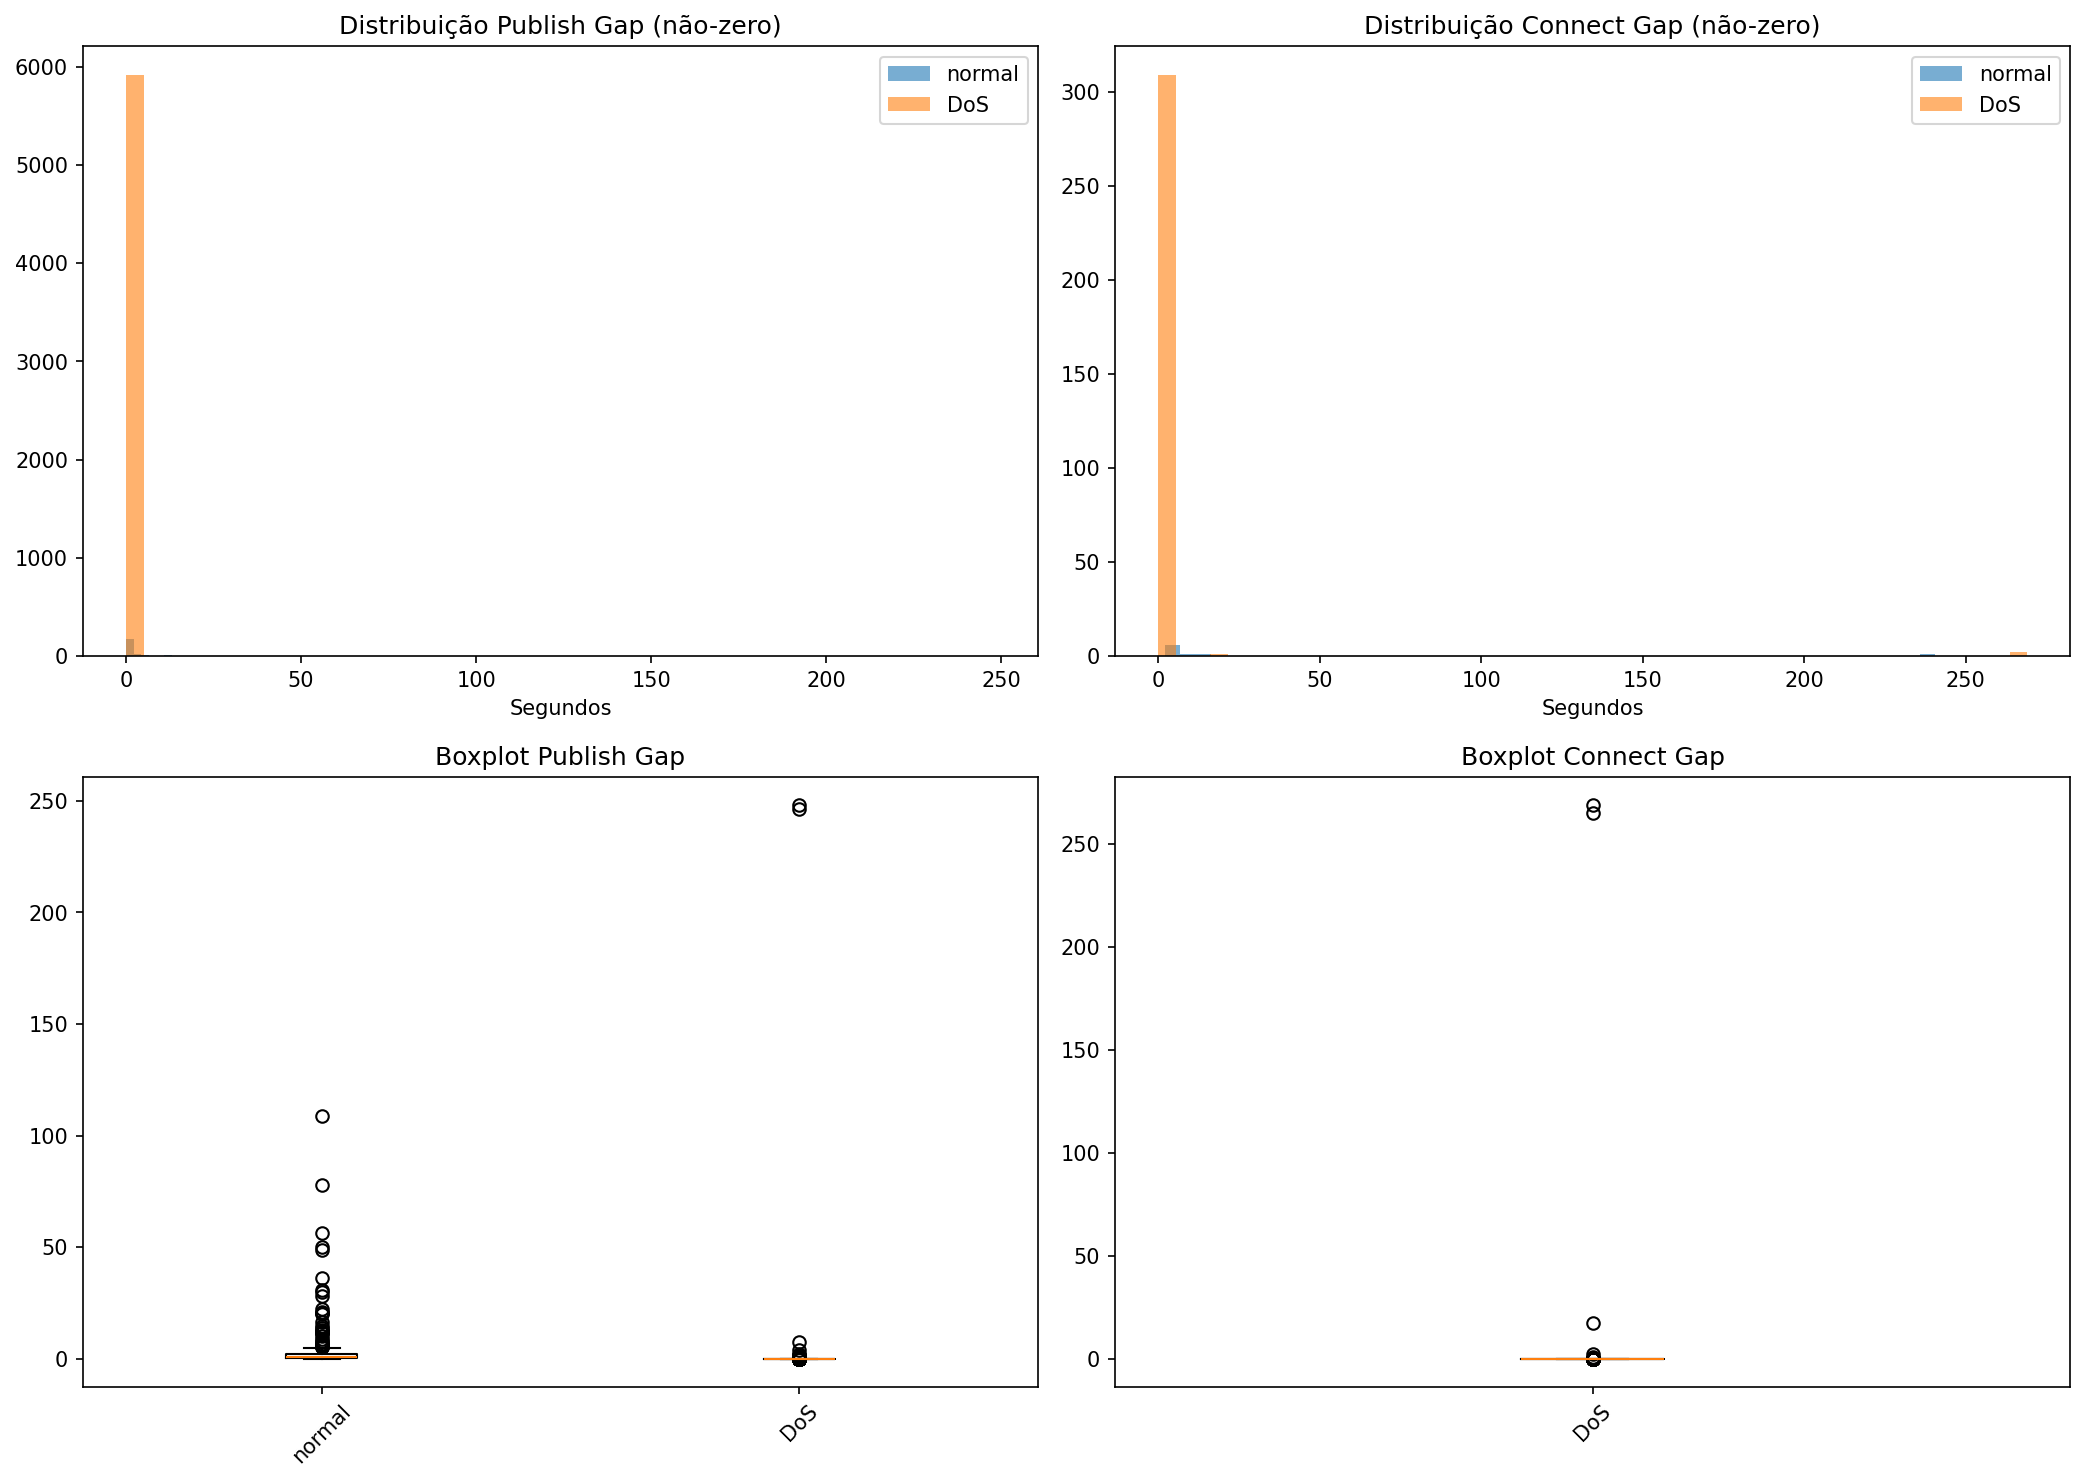
\includegraphics[width=0.9\textwidth]{reports_refactored/gap_features_distribution.png}
\caption{Distribuicao das features temporais publish\_gap e connect\_gap por classe de trafego.}
\end{figure}

\begin{figure}[H]
\centering
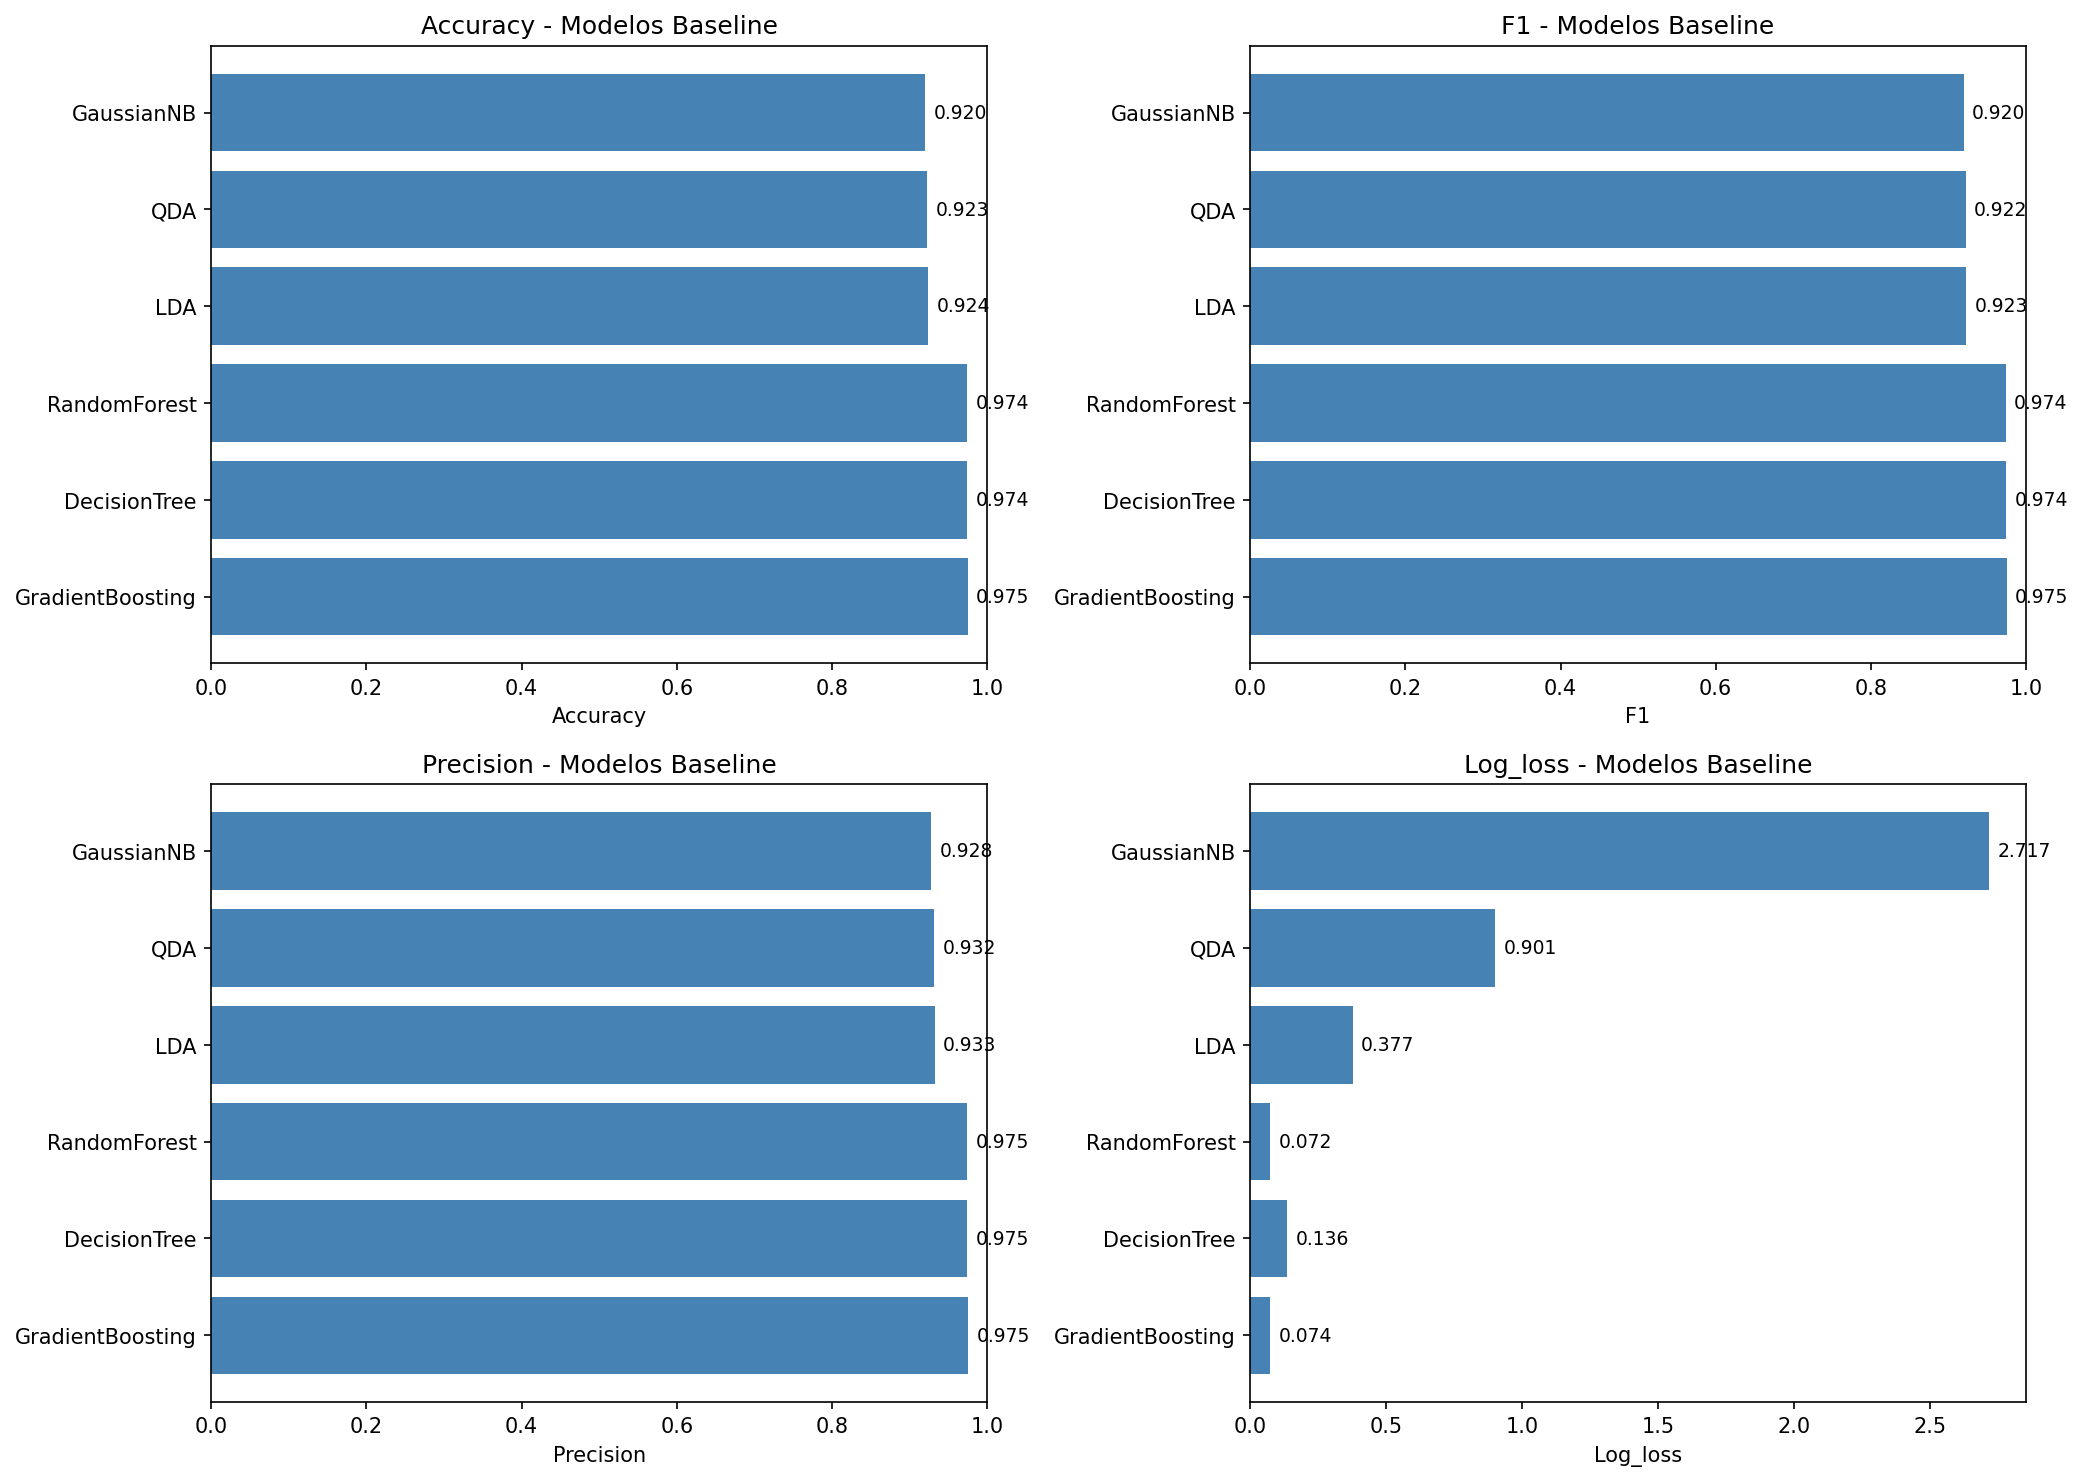
\includegraphics[width=0.8\textwidth]{reports_refactored/baseline_comparison.png}
\caption{Comparacao das metricas dos modelos baseline.}
\end{figure}

\begin{figure}[H]
\centering
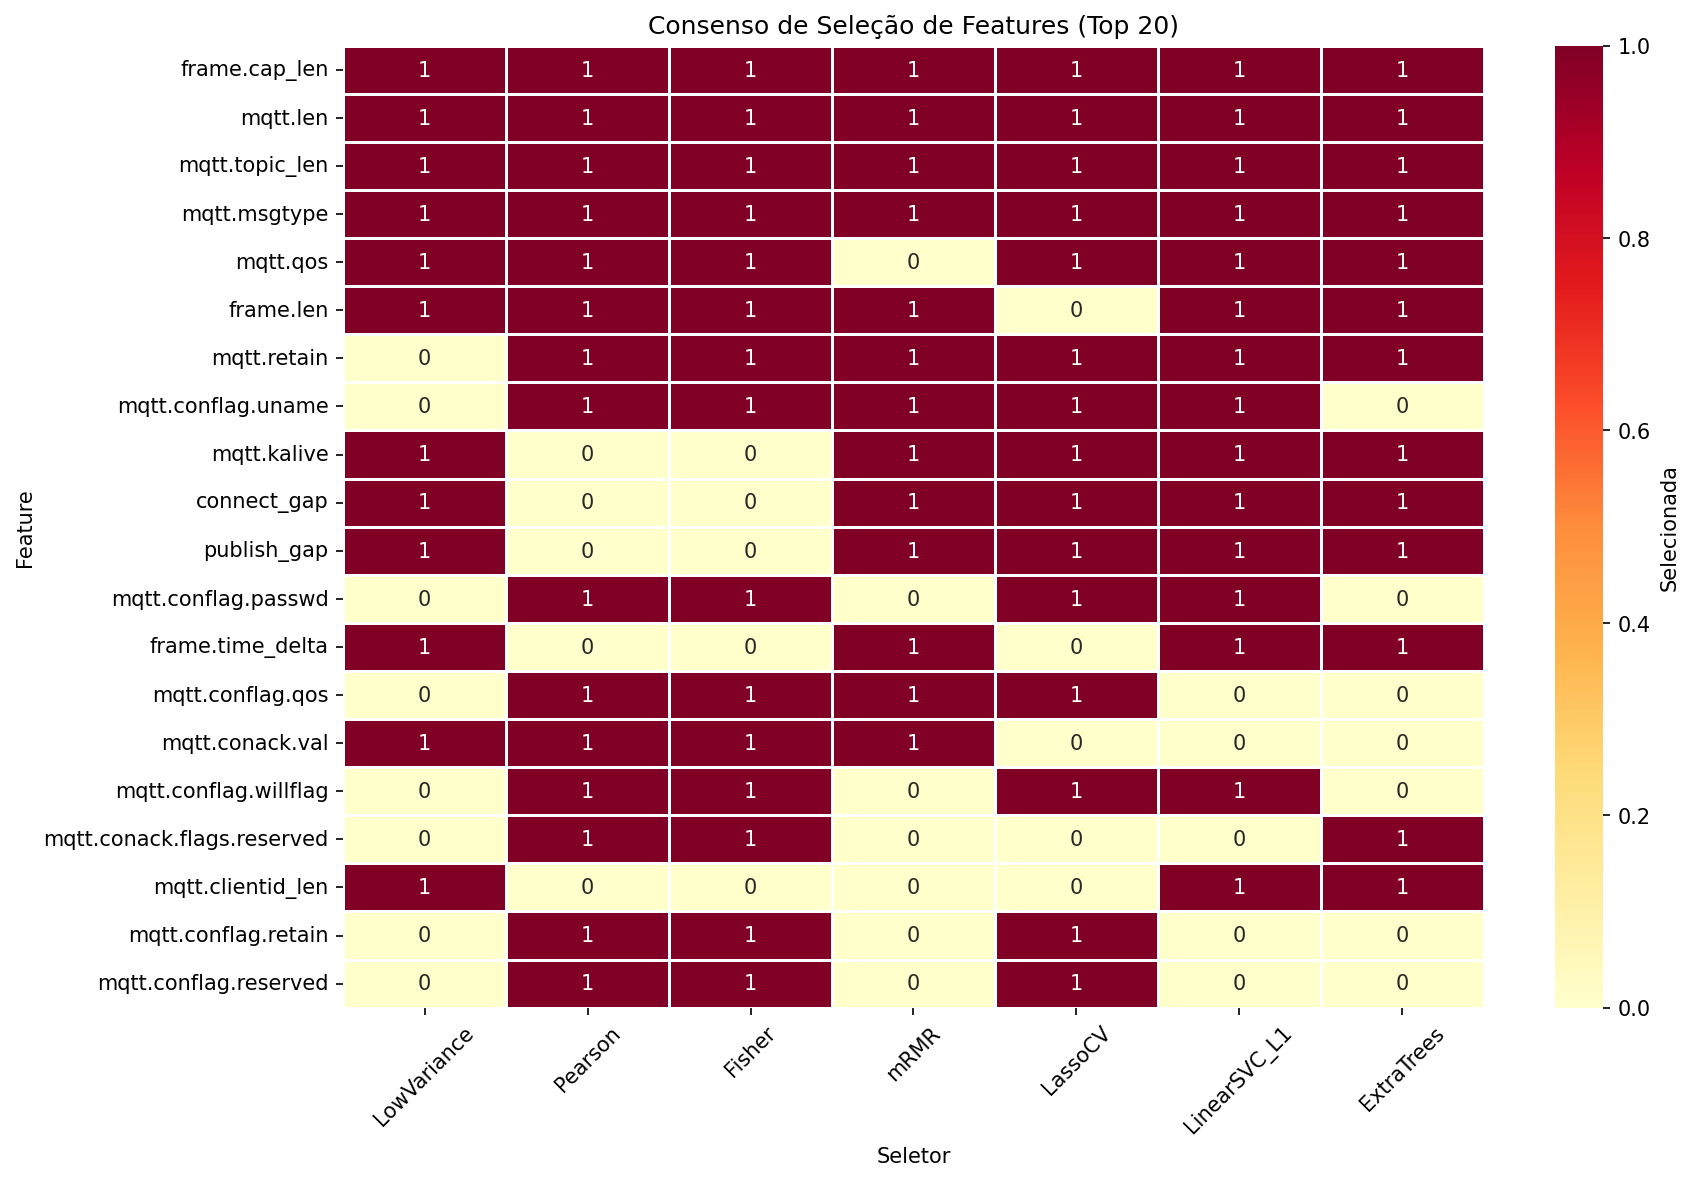
\includegraphics[width=0.85\textwidth]{reports_refactored/feature_consensus_heatmap.png}
\caption{Heatmap de consenso de selecao de features entre os metodos.}
\end{figure}

\begin{figure}[H]
\centering
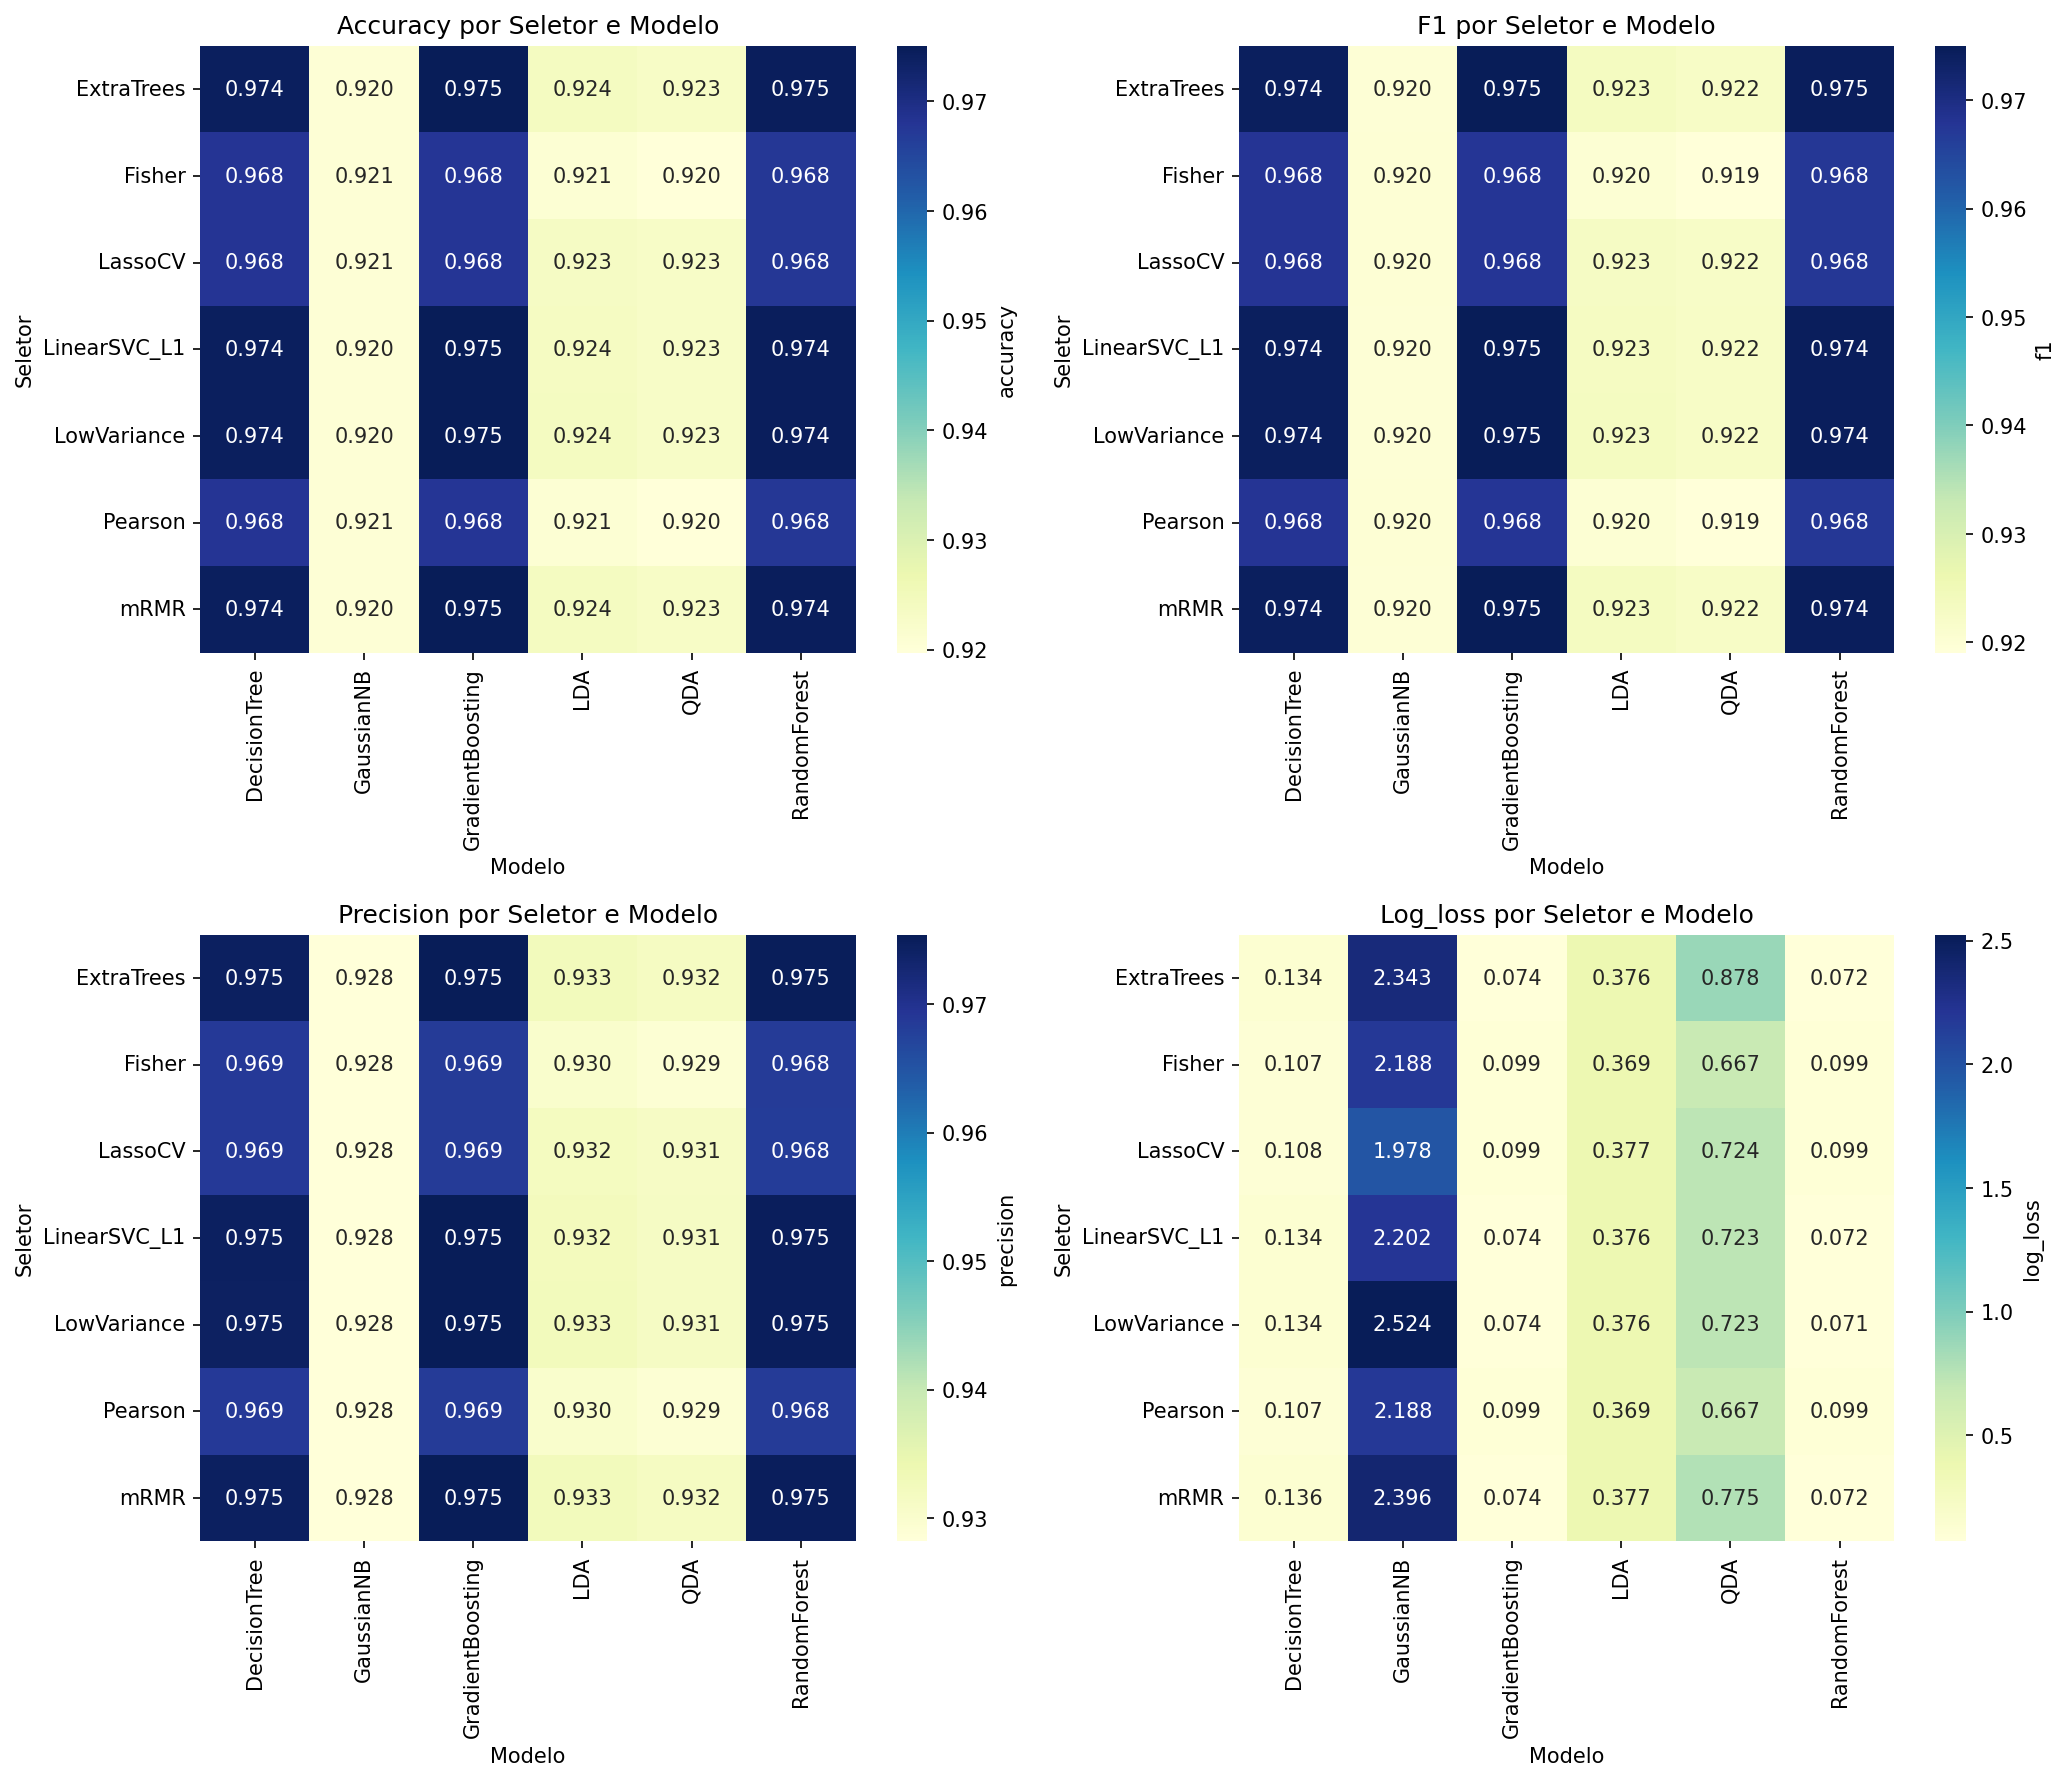
\includegraphics[width=0.85\textwidth]{reports_refactored/selection_heatmap.png}
\caption{Heatmap de desempenho por seletor de features e por modelo.}
\end{figure}

\begin{figure}[H]
\centering
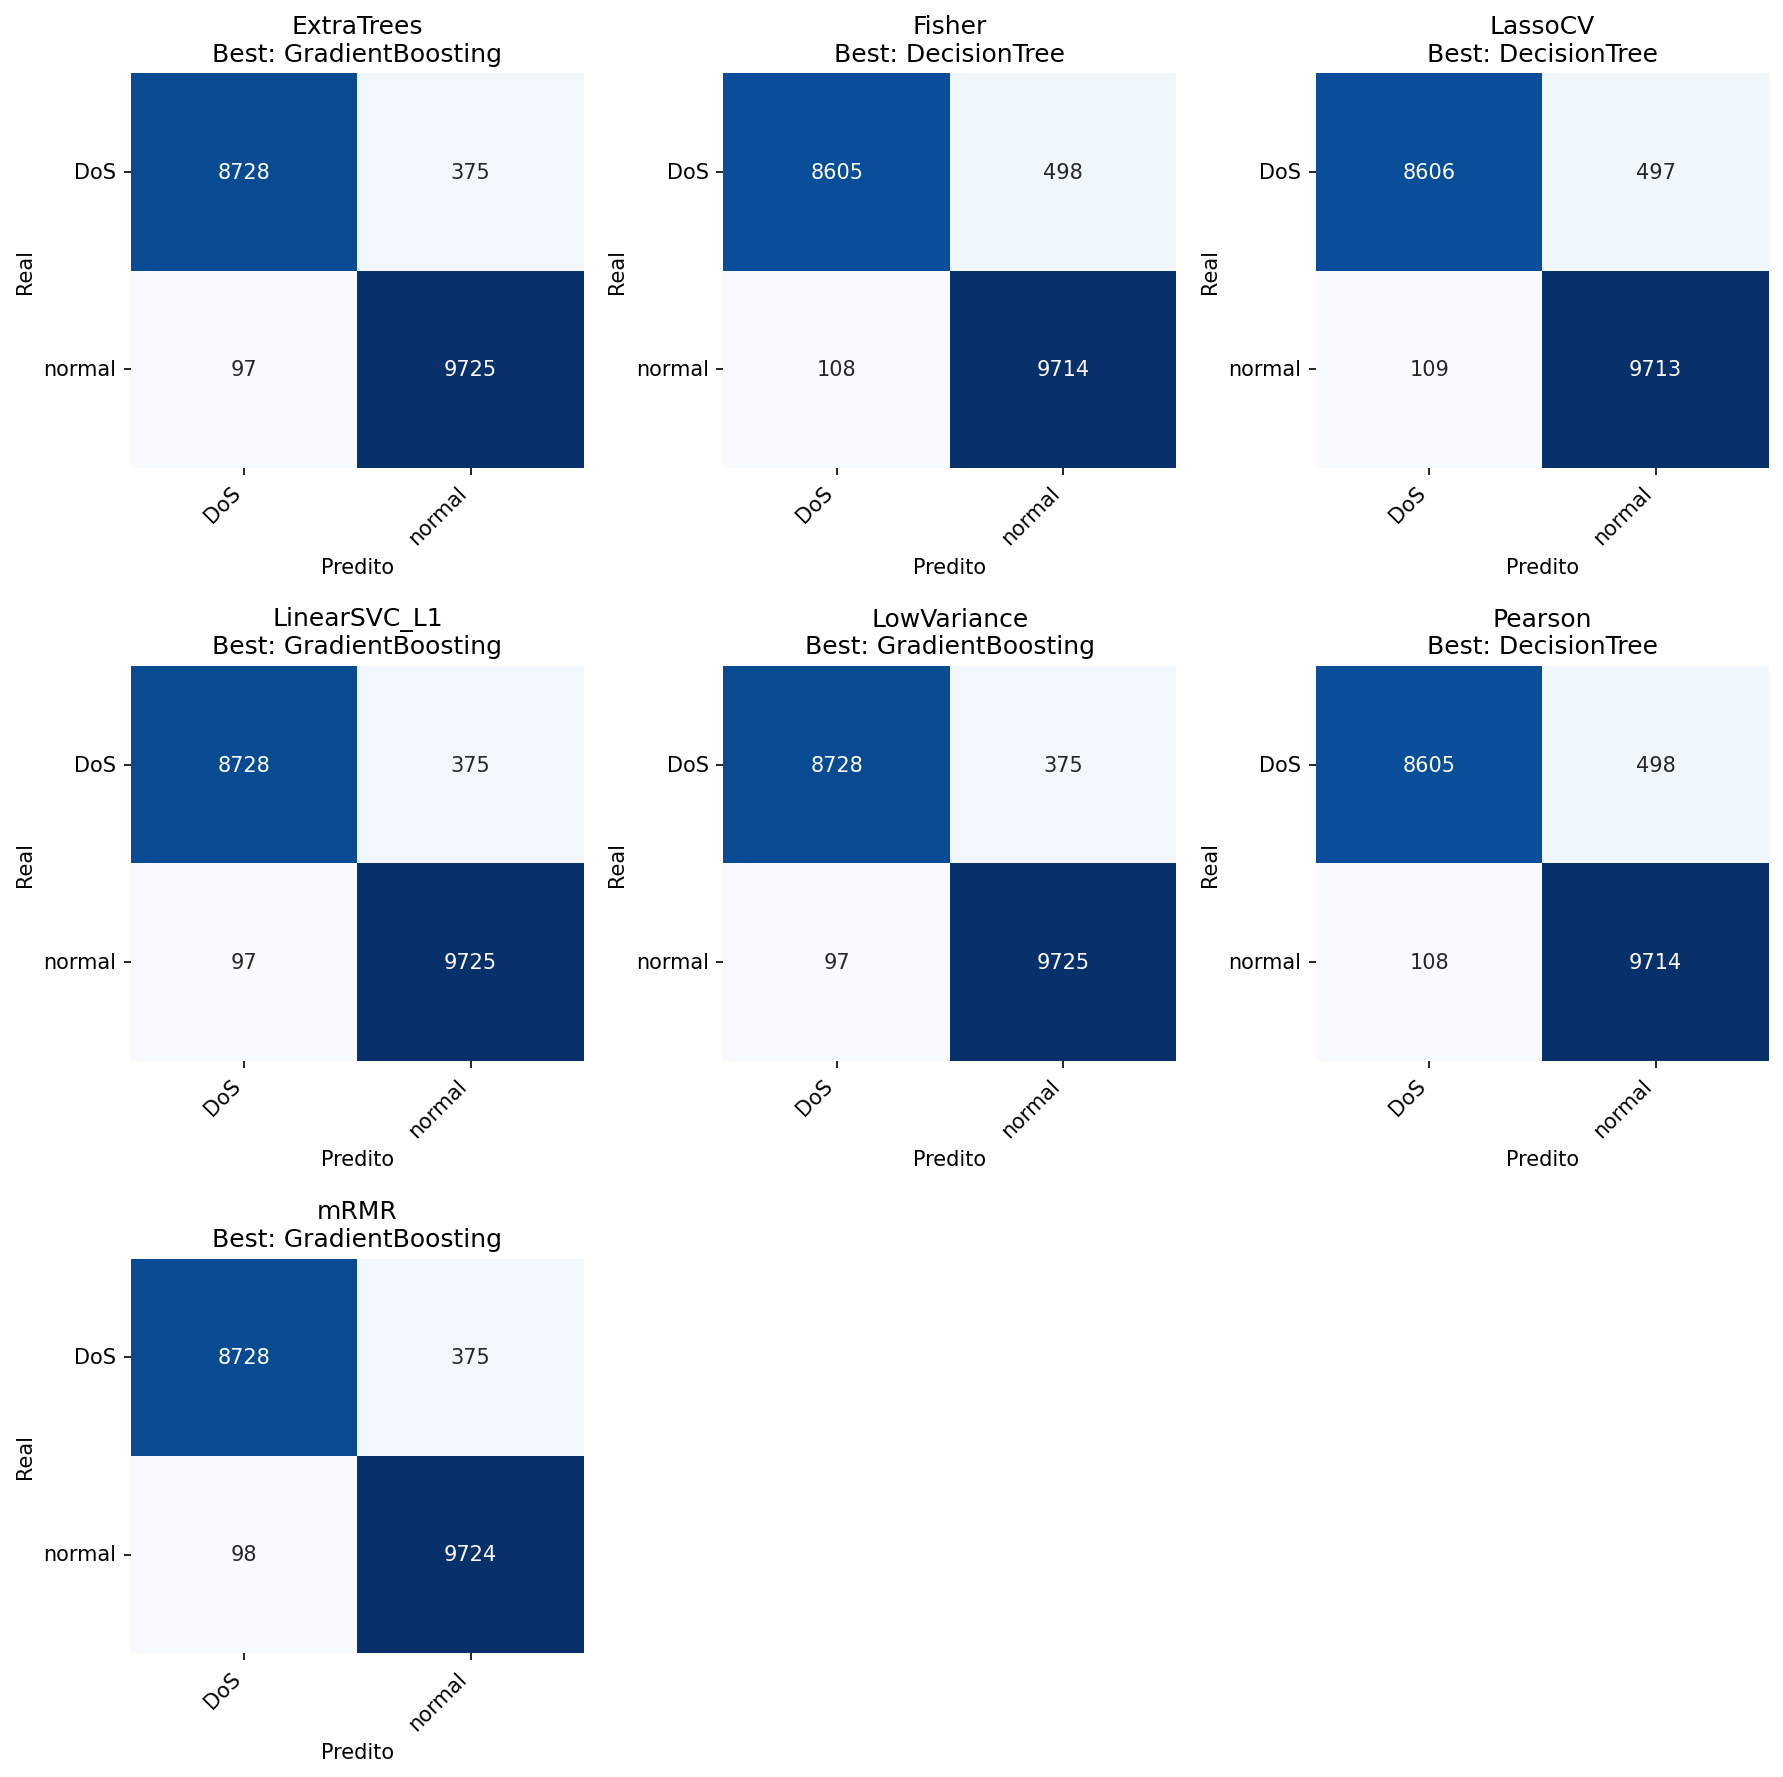
\includegraphics[width=0.9\textwidth]{reports_refactored/best_confusion_by_selector.png}
\caption{Matrizes de confusao dos melhores modelos para cada seletor de features.}
\end{figure}

\begin{figure}[H]
\centering
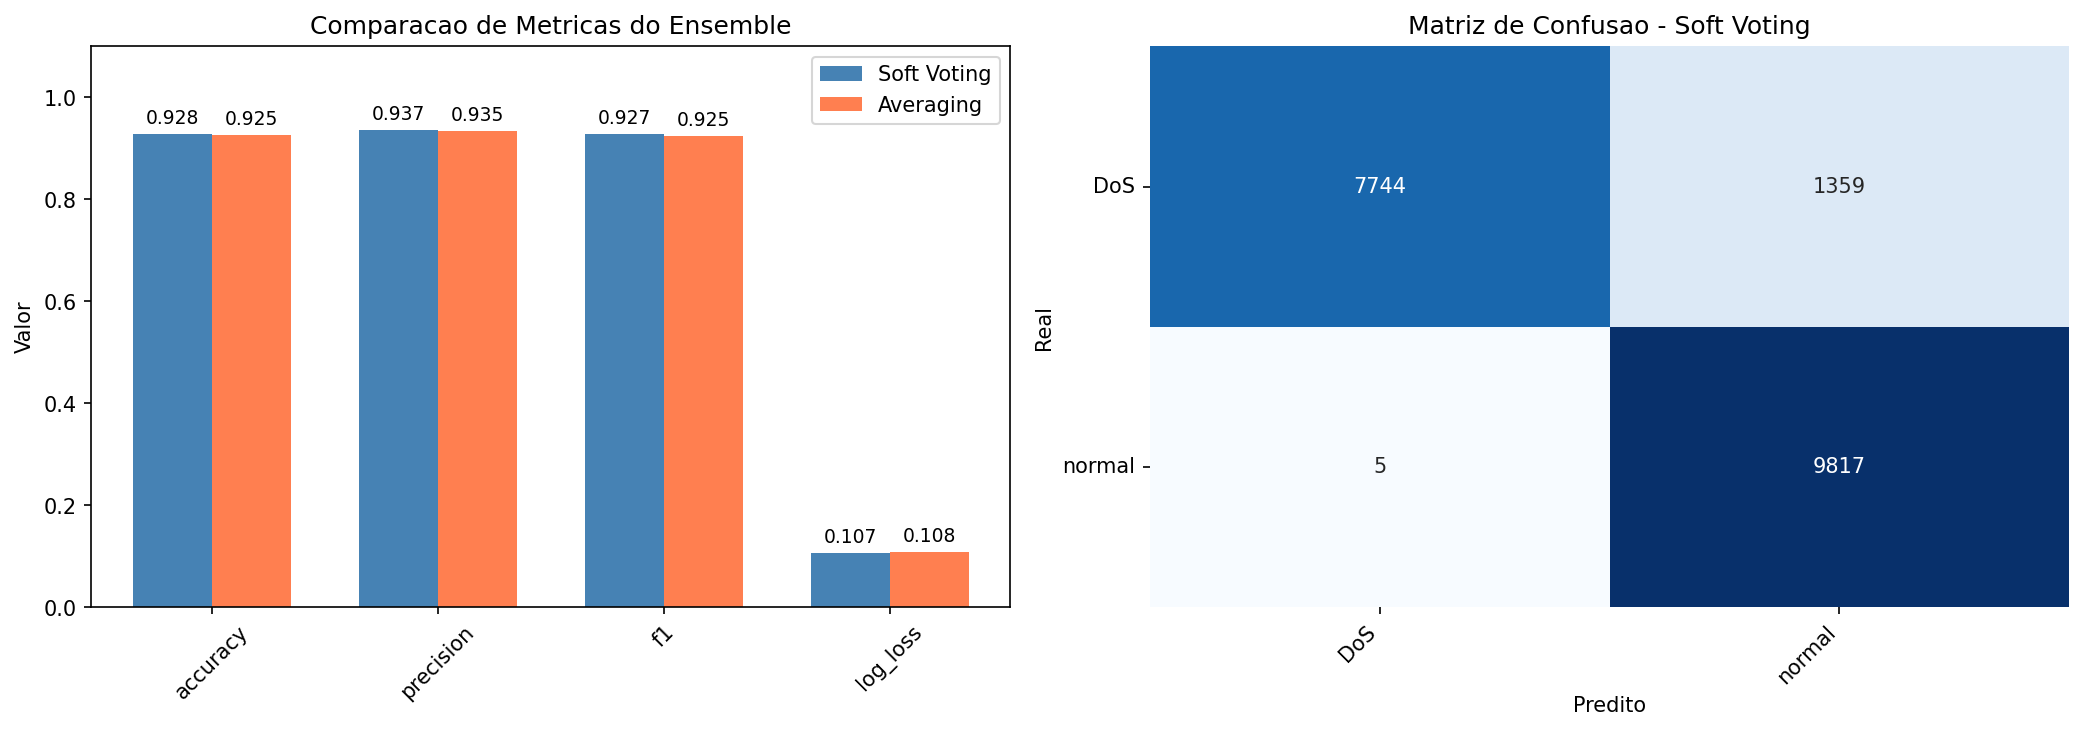
\includegraphics[width=0.9\textwidth]{reports_refactored/ensemble_comparison.png}
\caption{Comparacao de metricas no ensemble e matriz de confusao do Soft Voting.}
\end{figure}

\begin{figure}[H]
\centering
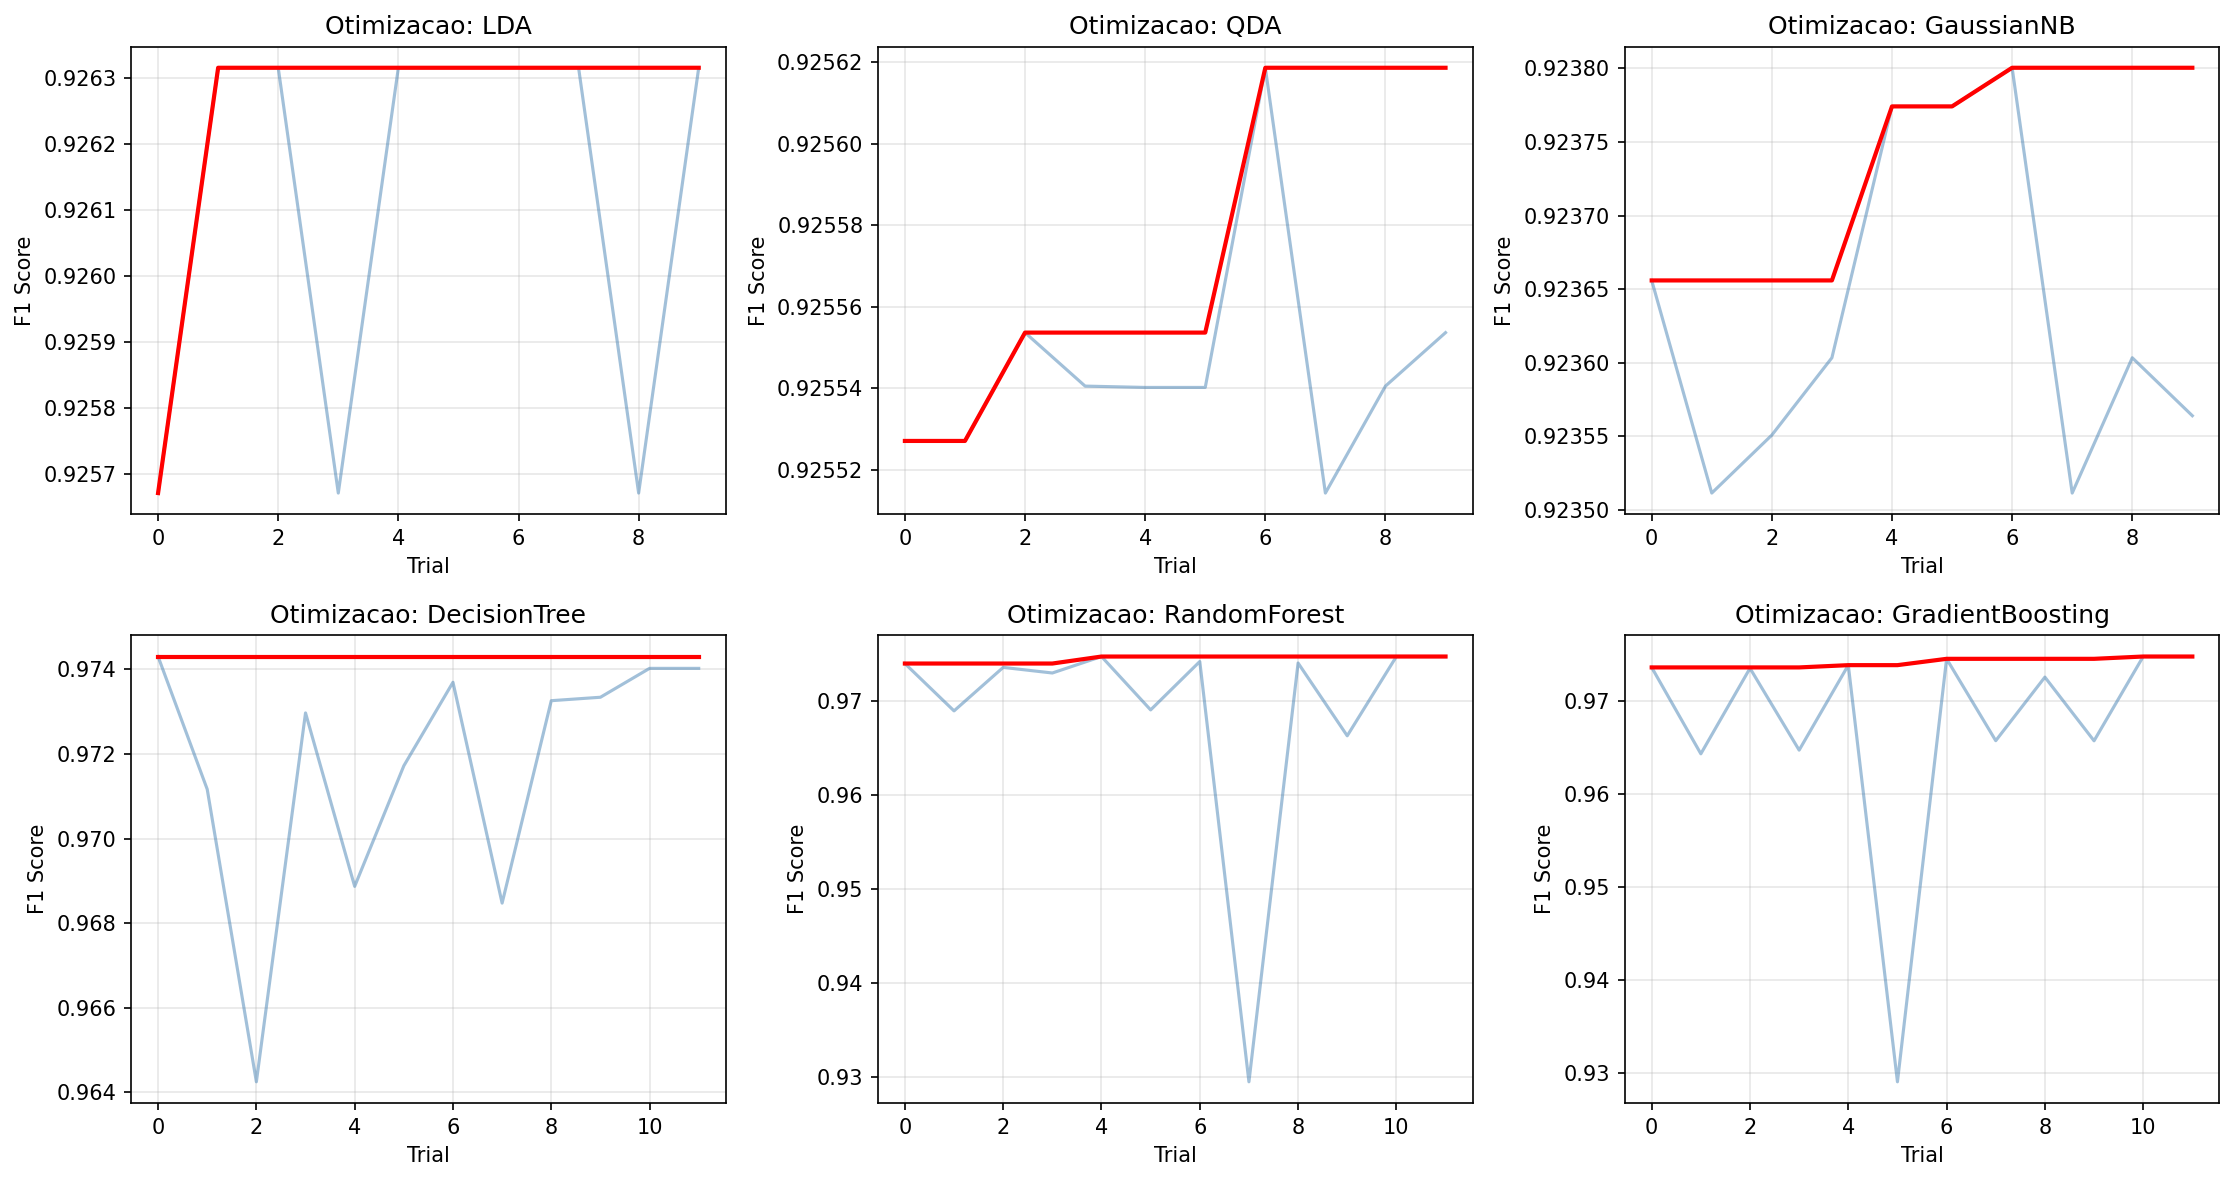
\includegraphics[width=0.9\textwidth]{reports_refactored/optuna_optimization_history.png}
\caption{Historico de convergencia da otimização por modelo no Optuna.}
\end{figure}

\begin{figure}[H]
\centering
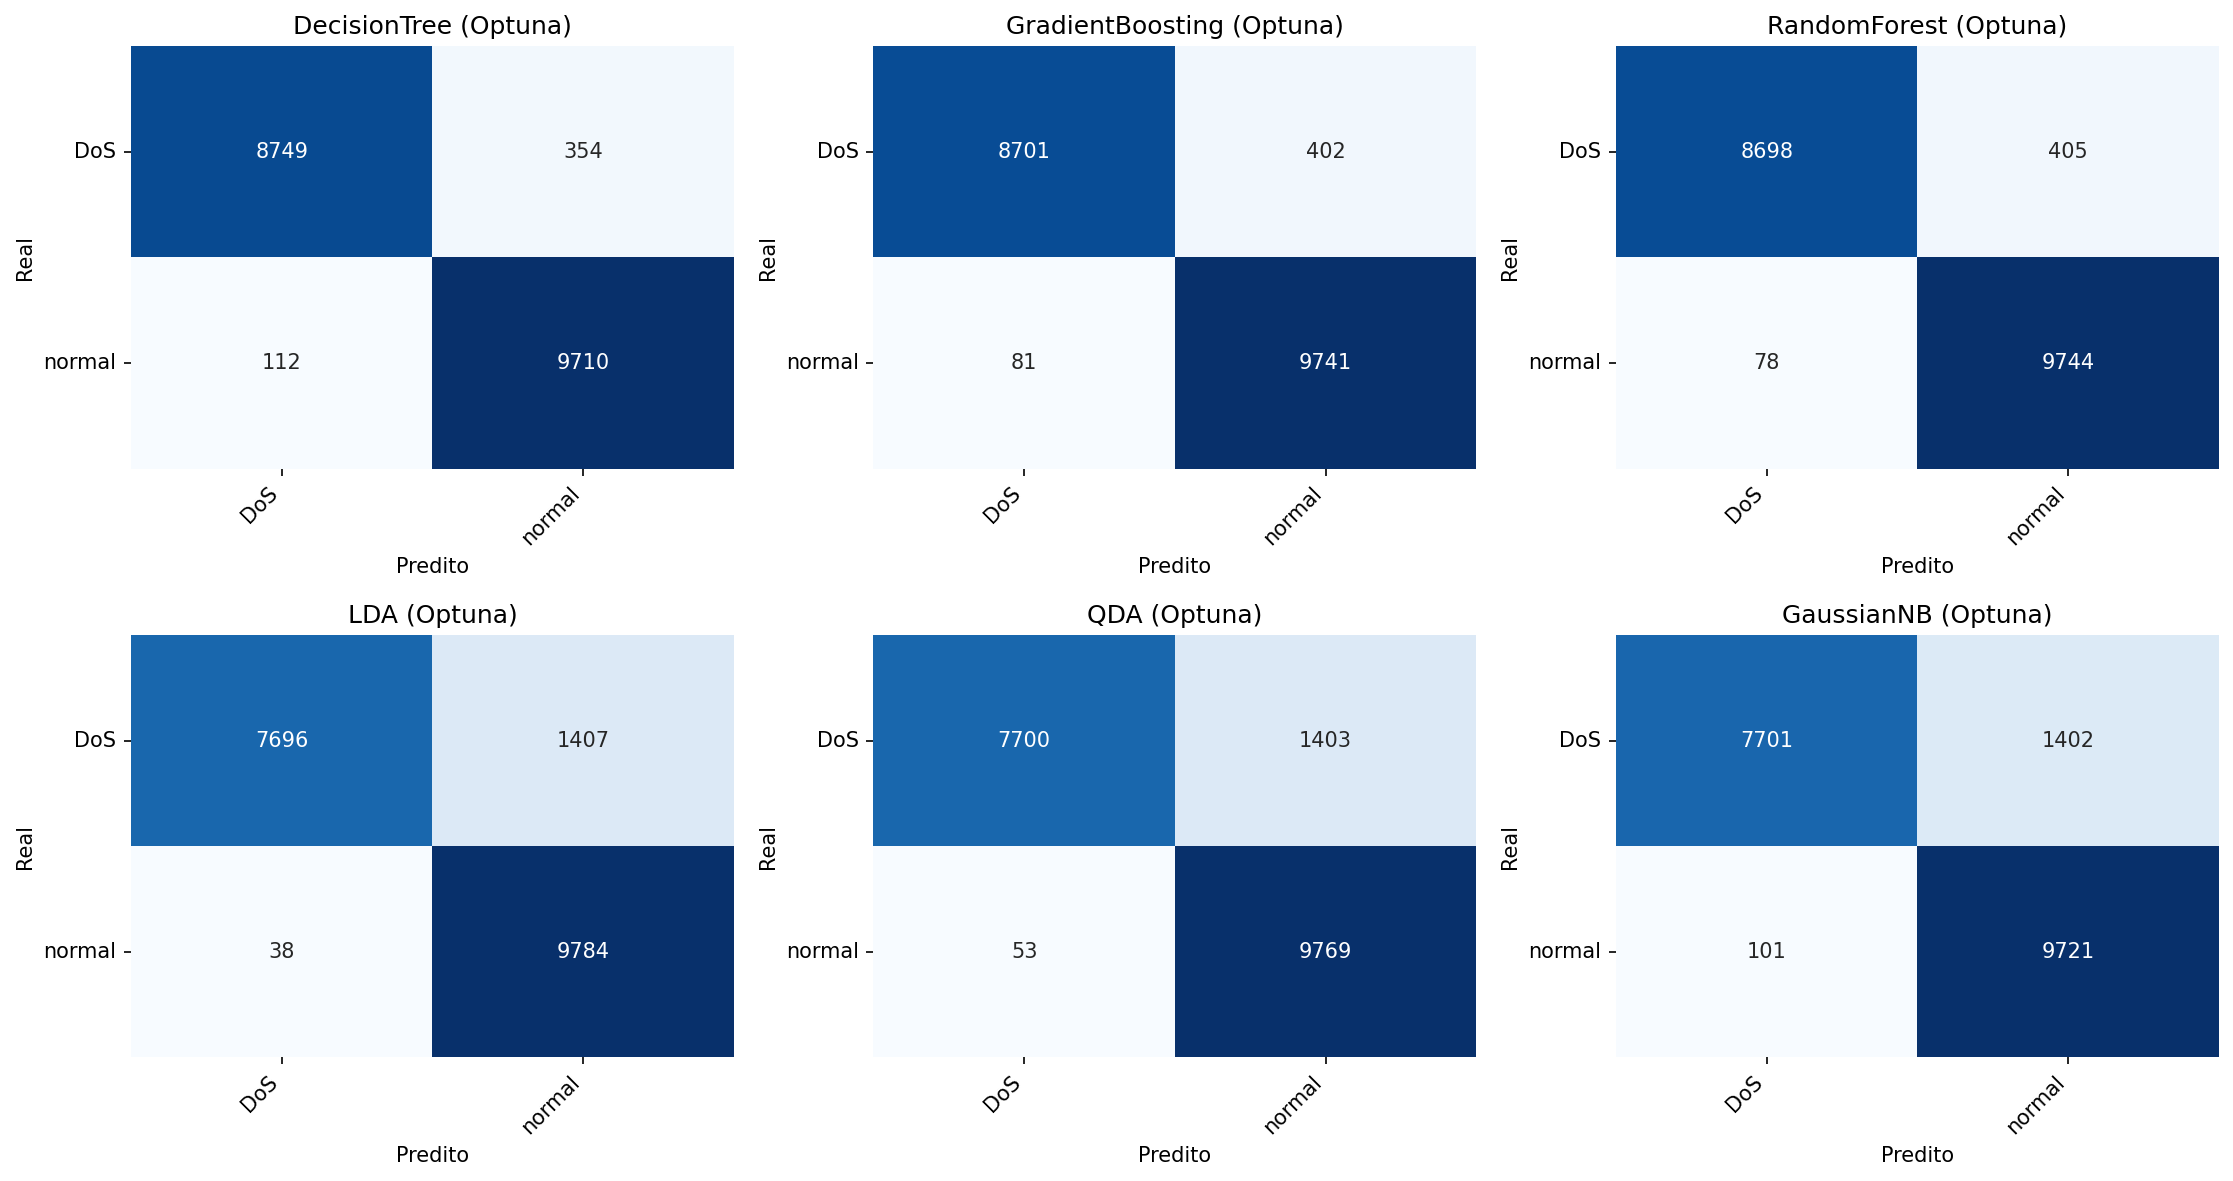
\includegraphics[width=0.9\textwidth]{reports_refactored/optuna_confusion_matrices.png}
\caption{Matrizes de confusao dos modelos otimizados no Optuna.}
\end{figure}

\begin{figure}[H]
\centering
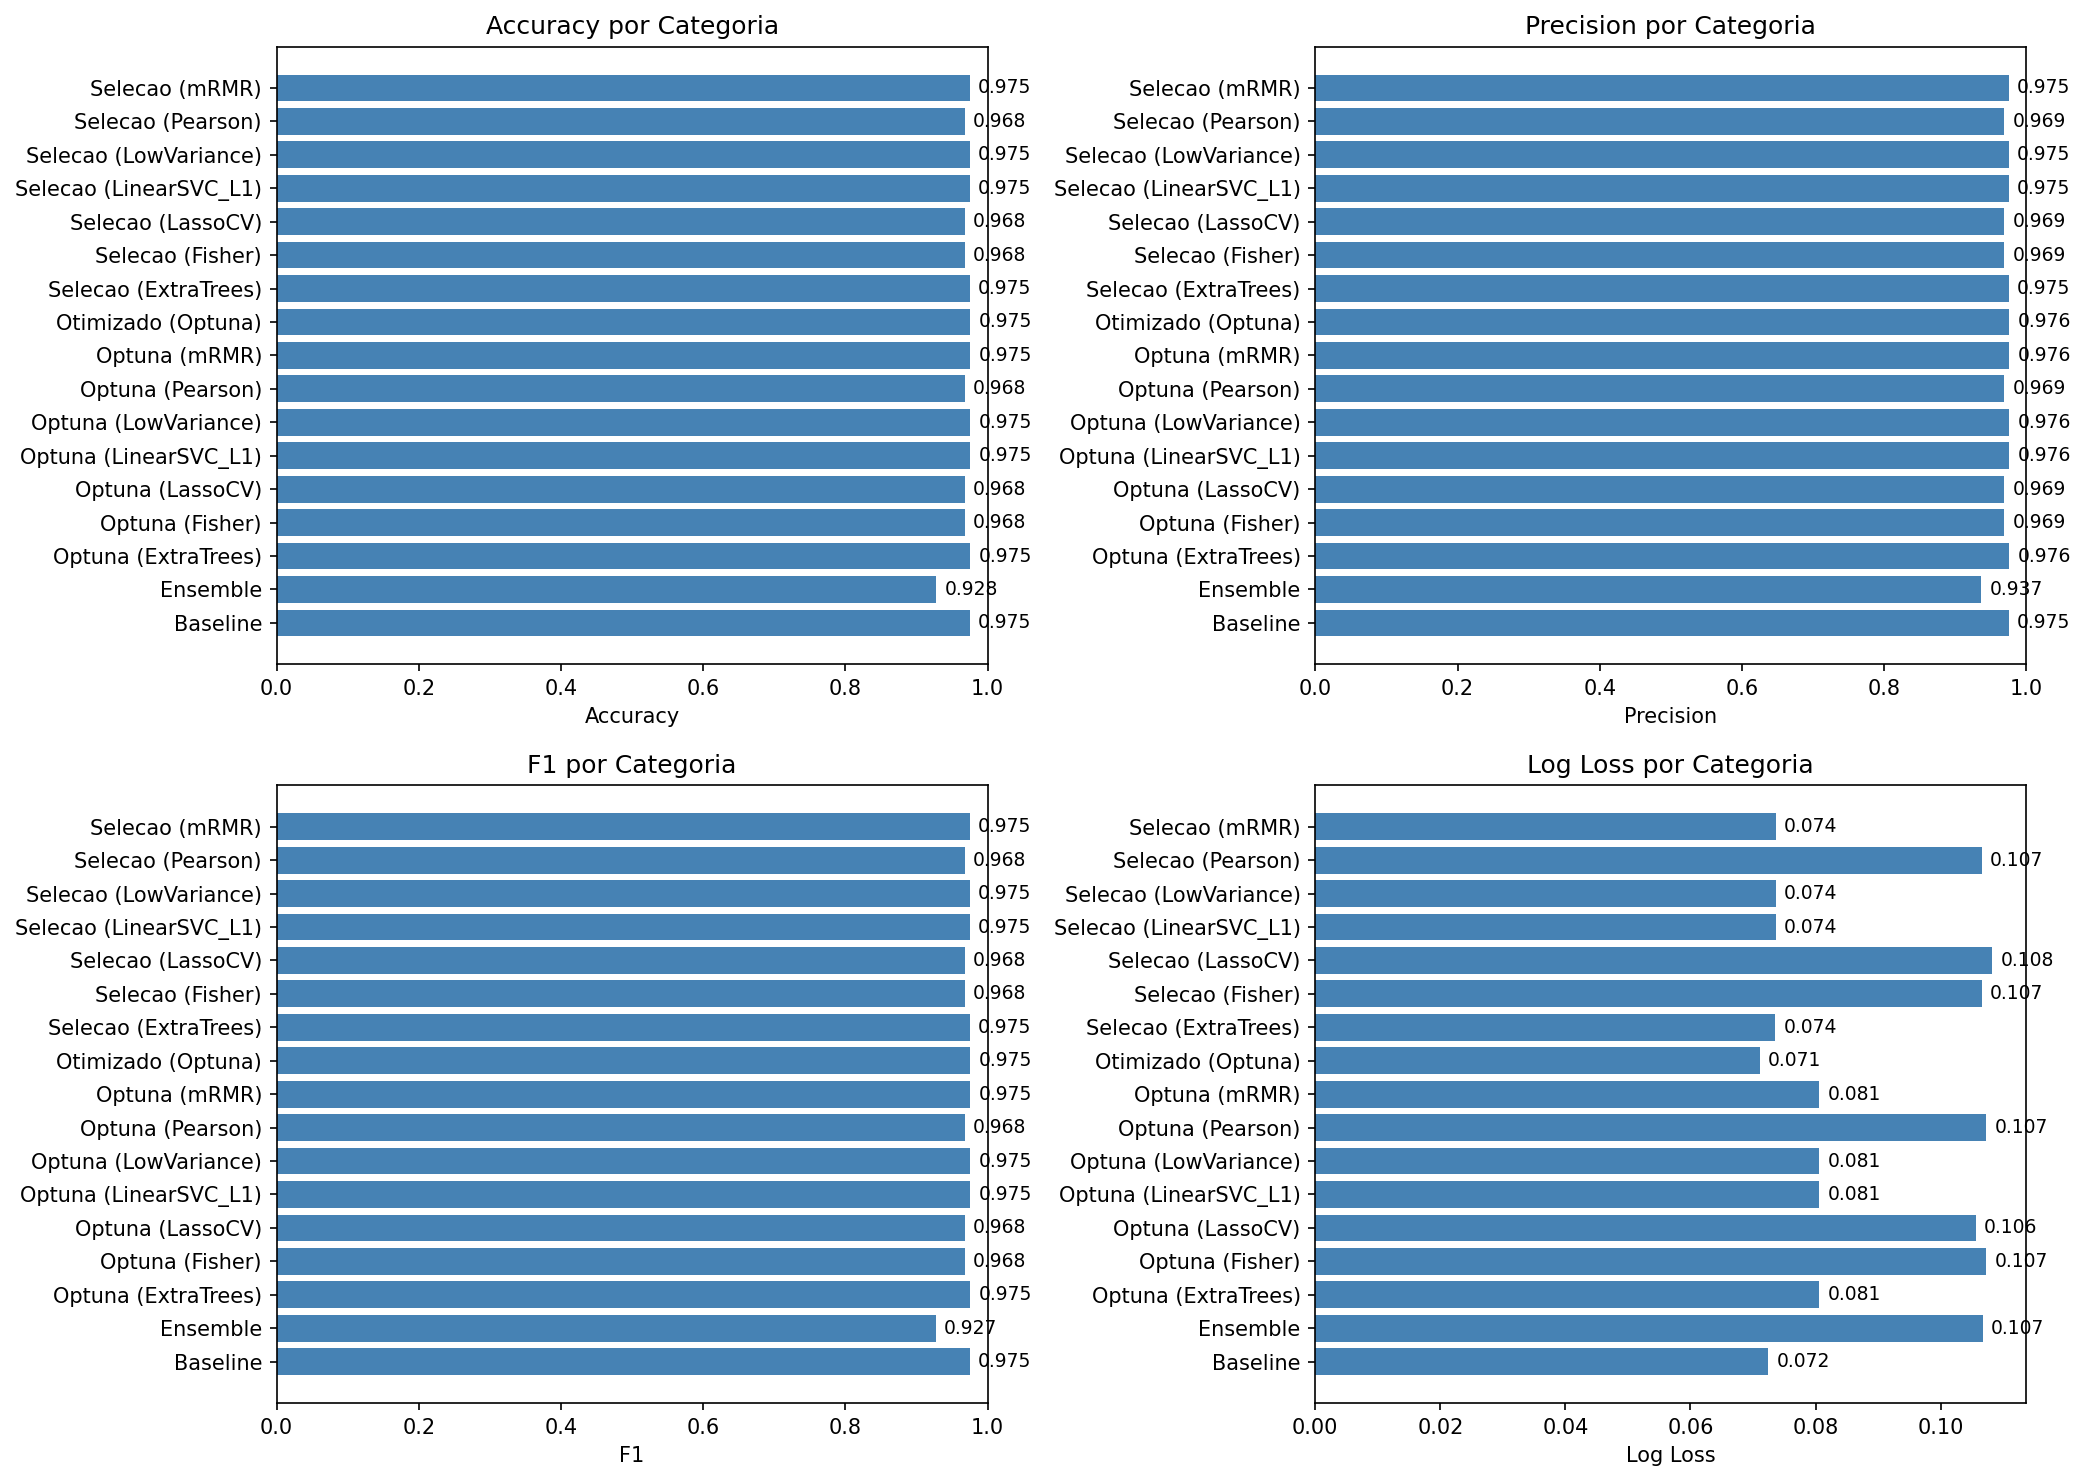
\includegraphics[width=0.85\textwidth]{reports_refactored/final_comparison.png}
\caption{Comparacao final das melhores metricas por categoria experimental.}
\end{figure}

\section{Saidas Textuais e Logs Principais}

\subsection{Log principal do baseline}
\begin{lstlisting}[style=plainlog]
Avaliando modelos baseline...

Treinando GradientBoosting...
  Accuracy:  0.9751
  Precision: 0.9754
  F1 Score:  0.9750
  Log Loss:  0.0736

Treinando DecisionTree...
  Accuracy:  0.9743
  Precision: 0.9746
  F1 Score:  0.9743
  Log Loss:  0.1359
\end{lstlisting}

\subsection{Log principal da selecao de features}
\begin{lstlisting}[style=plainlog]
Modelos avaliados com selecao de features: ['LDA', 'QDA', 'GaussianNB', 'DecisionTree', 'RandomForest', 'GradientBoosting']

Seletor: ExtraTrees (15 features)
  GradientBoosting: Acc=0.9751, Prec=0.9754, F1=0.9750, LogLoss=0.0736
  Melhor modelo do seletor: GradientBoosting (F1=0.9750)

Matrizes de confusao por seletor geradas (todos os modelos + melhor por seletor)
\end{lstlisting}

\subsection{Log principal do ensemble}
\begin{lstlisting}[style=plainlog]
ENSEMBLE - SOFT VOTING (PONDERADO)
Metricas Soft Voting:
  accuracy: 0.9279
  precision: 0.9366
  f1: 0.9274
  log_loss: 0.1067

ENSEMBLE - AVERAGING
Metricas Averaging:
  accuracy: 0.9255
  precision: 0.9346
  f1: 0.9249
  log_loss: 0.1085
\end{lstlisting}

\subsection{Log principal da otimizacao Optuna}
\begin{lstlisting}[style=plainlog]
Otimizando hiperparametros com budget reduzido por modelo...
- Otimizando LDA (n_trials=10)
  Melhor F1 (CV): 0.9263
  Melhores params: {'solver': 'svd'}
- Otimizando RandomForest (n_trials=12)
  Melhor F1 (CV): 0.9747
  Melhores params: {'n_estimators': 116, 'max_depth': 10, 'min_samples_split': 8, 'min_samples_leaf': 1}
Todos os modelos foram otimizados com sucesso.
\end{lstlisting}

\subsection{Log principal da consolidacao final}
\begin{lstlisting}[style=plainlog]
MELHOR MODELO IDENTIFICADO
Categoria: Otimizado (Optuna)
Modelo: DecisionTree (Optuna)
Metricas:
  Acuracia:  0.9754
  Precisao:  0.9757
  F1 Score:  0.9754
  Log Loss:  0.0806
\end{lstlisting}

\section{Exportacao Completa de Arquivos de Saida}

Para manter reprodutibilidade e auditoria integral, as saidas textuais e tabulares completas foram preservadas abaixo em formato literal.

\lstinputlisting[style=plainlog,caption={CSV completo de baseline.}]{reports_refactored/baseline_results.csv}
\lstinputlisting[style=plainlog,caption={CSV completo de selecao de features.}]{reports_refactored/selection_results.csv}
\lstinputlisting[style=plainlog,caption={CSV completo de ensemble.}]{reports_refactored/ensemble_results.csv}
\lstinputlisting[style=plainlog,caption={CSV completo de Optuna.}]{reports_refactored/optuna_results.csv}
\lstinputlisting[style=plainlog,caption={CSV completo de consolidacao final.}]{reports_refactored/final_results_all_models.csv}
\lstinputlisting[style=plainlog,caption={Resumo de melhores hiperparametros por modelo no Optuna.}]{reports_refactored/optuna_best_params_summary.csv}
\lstinputlisting[style=plainlog,caption={Matriz do melhor modelo por seletor.}]{reports_refactored/best_confusion_matrix_by_selector.json}
\lstinputlisting[style=plainlog,caption={Matrizes dos modelos otimizados no Optuna.}]{reports_refactored/optuna_confusion_matrices.json}

\end{document}
